\documentclass[tikz,border=4pt]{standalone}
% Paleta y fuentes compartidas por el libro y las figuras (única fuente de verdad).
\RequirePackage{xcolor}
\definecolor{oxido}{HTML}{B7410E}
\definecolor{cobre}{HTML}{D27D2D}
\definecolor{carbon}{HTML}{2B2B2B}
\definecolor{azul}{HTML}{1F5F8B}
\definecolor{arena}{HTML}{F4EDE4}

\usepackage{fontspec}
\setsansfont{FiraSans}[Extension=.otf,UprightFont=*-Regular,BoldFont=*-SemiBold,ItalicFont=*-Italic,BoldItalicFont=*-SemiBoldItalic]
\setmonofont{FiraMono}[Extension=.otf,UprightFont=*-Regular,BoldFont=*-Medium,Scale=0.95]
\usetikzlibrary{positioning,arrows.meta,calc,decorations.pathreplacing}
\newcommand{\tit}{\sffamily\small\bfseries}
\newcommand{\cod}{\ttfamily\scriptsize\color{carbon!80}}
\begin{document}
\sffamily\small
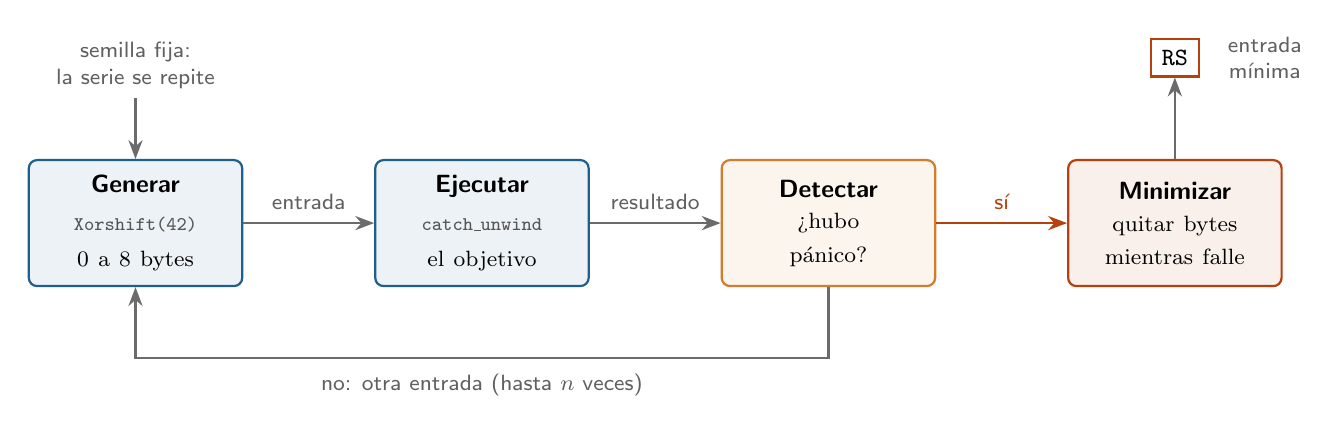
\begin{tikzpicture}[>={Stealth[length=2.4mm]},
  paso/.style={draw=#1,fill=#1!8,line width=0.8pt,rounded corners=3pt,
    text width=2.5cm,minimum height=1.6cm,align=center,inner sep=3pt,
    execute at begin node={\hyphenpenalty=10000}},
  nota/.style={font=\sffamily\footnotesize,text=carbon!75,align=center},
  flecha/.style={->,thick,carbon!70}]
  \node[paso=azul] (gen) at (0,0) {{\tit Generar}\\[2pt]{\cod Xorshift(42)}\\[1pt]{\footnotesize 0 a 8 bytes}};
  \node[paso=azul] (eje) at (4.4,0) {{\tit Ejecutar}\\[2pt]{\cod catch\_unwind}\\[1pt]{\footnotesize el objetivo}};
  \node[paso=cobre] (det) at (8.8,0) {{\tit Detectar}\\[2pt]{\footnotesize ¿hubo\\pánico?}};
  \node[paso=oxido] (min) at (13.2,0) {{\tit Minimizar}\\[2pt]{\footnotesize quitar bytes\\mientras falle}};
  % Semilla y resultado
  \node[nota] (sem) at (0,2.0) {semilla fija:\\la serie se repite};
  \draw[flecha] (sem) -- (gen);
  \node[draw=oxido,line width=0.8pt,fill=white,font=\ttfamily\small,inner sep=4pt] (res) at (13.2,2.1) {RS};
  \node[nota,anchor=west] at (13.75,2.1) {entrada\\mínima};
  \draw[flecha] (min) -- (res);
  % Flechas del ciclo
  \draw[flecha] (gen) -- node[nota,above=1pt] {entrada} (eje);
  \draw[flecha] (eje) -- node[nota,above=1pt] {resultado} (det);
  \draw[flecha,oxido] (det) -- node[nota,above=1pt,text=oxido] {sí} (min);
  \draw[flecha] (det.south) -- ++(0,-0.9) -| node[nota,pos=0.25,below=2pt] {no: otra entrada (hasta $n$ veces)} (gen.south);
\end{tikzpicture}
\end{document}
